\subsection{Optimización de Hiperparámetros}
La optimización de hiperparámetros se refiere al proceso de ajustar los parámetros 
de entrenamento y configuracion de un modelo de Machine Learning con el objetivo de 
mejorar su desempeño. Los hiperparámetros son variables que no se aprenden automáticamente 
a partir de los datos, sino que deben ser configurados por el investigador.\medskip

En un modelo de Machine Learning, los hiperparámetros pueden incluir variables como 
la tasa de aprendizaje, la profundidad de la red neuronal, la cantidad de neuronas en 
cada capa, el tamaño del Batch, entre otros. El proceso de optimización implica la 
selección cuidadosa de los valores de los hiperparámetros que maximicen el rendimiento 
del modelo en un conjunto de datos de prueba. Esto generalmente se realiza mediante 
la búsqueda de un rango de valores posibles para los hiperparámetros y evaluando el 
rendimiento del modelo en cada combinación posible.\medskip

La optimización de hiperparámetros es un aspecto importante del desarrollo de modelos 
, ya que una mala selección de hiperparámetros puede llevar a un modelo con un rendimiento 
deficiente. Un modelo que esté bien optimizado puede mejorar significativamente su 
capacidad para hacer predicciones precisas y generalizar a datos nuevos y desconocidos.

\subsubsection{Optimización de Hiperparámetros con Optimización Bayesiana}
La optimización bayesiana es un método de optimización de hiperparámetros para modelos 
de Machine Learniing que utiliza un enfoque probabilístico para buscar el conjunto 
óptimo de hiperparámetros. En lugar de evaluar todas las combinaciones posibles de 
hiperparámetros, la optimización bayesiana utiliza una estrategia de búsqueda más 
inteligente que utiliza la información de iteraciones anteriores para buscar en el 
espacio de búsqueda de manera más eficiente.\medskip

La optimización bayesiana comienza con una función subrogacion que mide la calidad del modelo 
en un conjunto de datos de prueba. La estrategia de optimización bayesiana consiste en construir 
un modelo probabilístico de la función objetivo y utilizarlo para decidir qué hiperparámetros 
probar a continuación. En cada iteración, el modelo actualizado sugiere un conjunto de 
hiperparámetros que se espera que tengan una buena probabilidad de mejorar el rendimiento 
del modelo. El modelo se entrena con los nuevos hiperparámetros y se evalúa 
su rendimiento en el conjunto de prueba. Esta evaluación se utiliza para actualizar el 
modelo probabilístico, y se repite el proceso de búsqueda de hiperparámetros hasta 
que se encuentra una combinación que satisfaga el criterio de parada.

\subsubsection{Aplicación de Optimización Bayesiana con Optuna}
Optuna utiliza el método de optimización bayesiana para buscar el conjunto óptimo de
hiperparámetros. Además, mediante Optuna-Dashboard se puede visualizar el proceso de
optimización, la importancia de cada hiperparámetro, la relación entre los hiperparámetros
y llevar un registro de las mejores combinaciones de hiperparámetros encontradas.\medskip

A continuación se muestra el listado de hiperparámetros:

\begin{table}[ht]
    \centering
    \begin{tabular}[ht]{l|c|c} 
        \textbf{Lista de Hyperparametros} & \textbf{Rango de valores} & \textbf{Valor Optimo}\\
        \hline
        \textbf{Número de instacias pequeñas} & 0 -- 20k & 20k\\
        \textbf{Número de instacias medianas} & 0 -- 20k & 10k\\
        \textbf{Número de instacias grandes}  & 0 -- 20k & 10k \\
        \textbf{Tasa de aprendizaje} & 0.00001 -- 0.001 & 15 \\
        \textbf{Número de épocas} & 5 -- 35 & 30 \\ 
        \textbf{Número de episodios} & 1 -- 3 & 2 \\
        \textbf{Tamaño del Batch} & 64, 128, 256 & 64\\
        \textbf{Canales ocultos} & 100 -- 300 & 200 \\
        \textbf{Número de capas ocultas} & 1 -- 6 & 1 \\
    \end{tabular}
    \caption{Lista de hiperparámetros}
    \label{tab:hyperparams}
\end{table}

Esta lista de hiperparámetros se obtuvo a partir de múltiples experimentos. En cada 
experimento se realizaban tres entrenamientos con los mismos hiperparámetros y luego
se promediaba el resultado de cada métrica, para así obtener un resultado más estable.
El objetivo de estos experimentos era minimizar la función opbjectivo y se realizaron
un total de 300 pruebas con diferentes combinaciones. En la figura \ref{fig:experiments}
se puede observar la visualización de los experimentos realizados y como progresa la
configuracion de los hiperparámetros, aqui los puntos azules representan los experimentos
realizados y la linea roja representa la mejor combinación de hiperparámetros encontrada
hasta el momento.

\begin{figure}[ht]
    \centering
    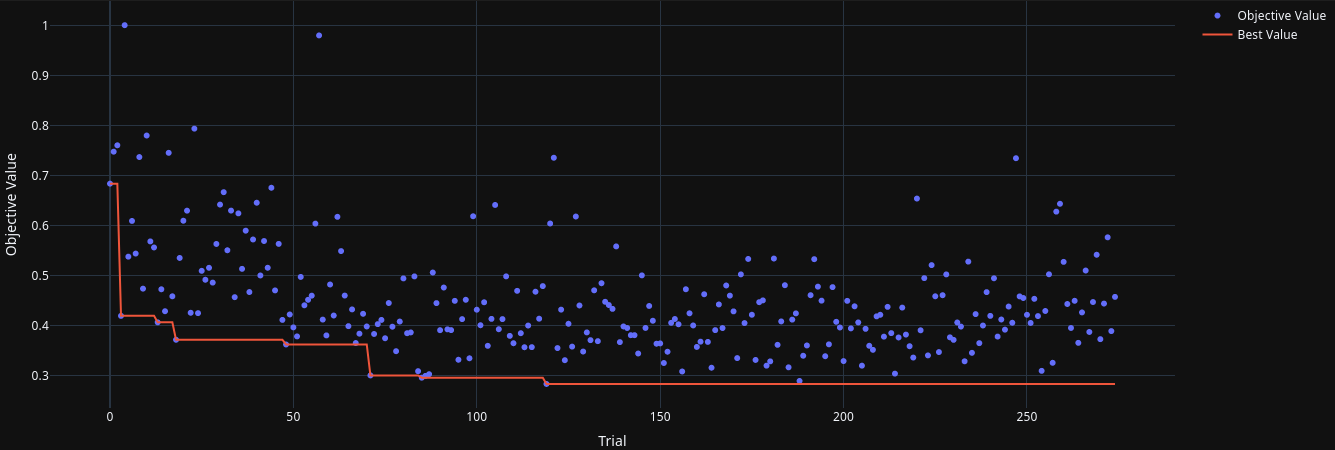
\includegraphics[scale=0.31]{experiments.png}
    \caption{Visualizacion de la experimentacion de hiperparámetros}
    \label{fig:experiments}
\end{figure}

Una de las ventajas de utilizar Optuna es que se puede visualizar la importancia de cada
hiperparámetro, en la figura \ref{fig:importance} se puede observar que los hiperparámetros
que mayor impacto tienen en el rendimiento del modelo son la tasa de aprendizaje, el número
de instacias pequeñas y el número de capas ocultas. Este conocimento ha traido consigo
una mejora en el rendimiento del modelo, en este caso debido a que se ha visto que el
número optimo de capas ocultas es 1, ha supuesto una mejora en la velocidad del modelo
ya que no solo se reduce el tiempo de entrenamiento sino que también se reduce el tiempo
de procedimiento a la hora de realizar predicciones.

\begin{figure}[ht!]
    \centering
    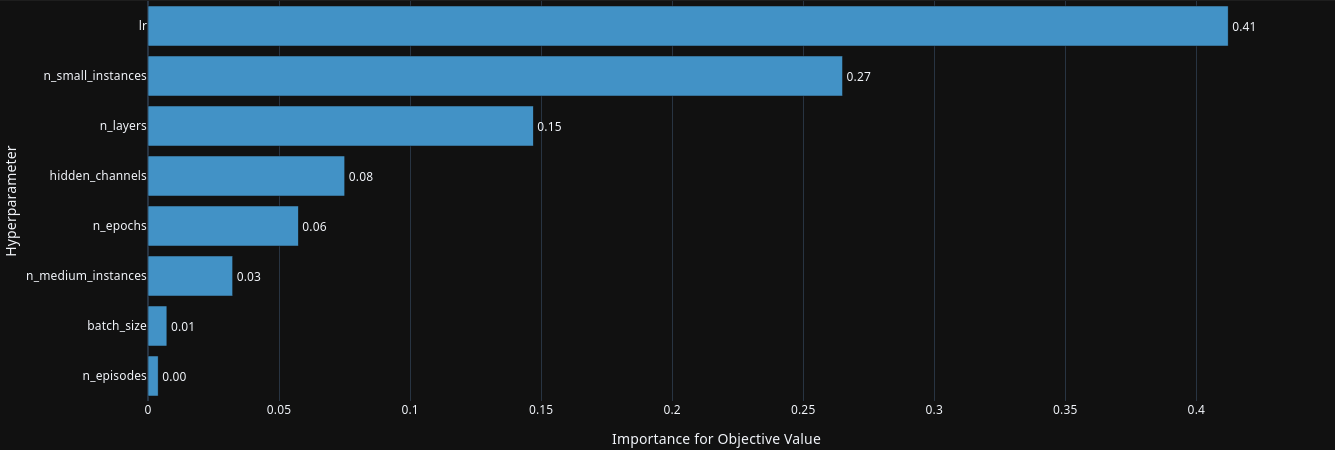
\includegraphics[scale=0.31]{importance.png}
    \caption{Importancia de los hiperparámetros}
    \label{fig:importance}
\end{figure}
